% Options for packages loaded elsewhere
\PassOptionsToPackage{unicode}{hyperref}
\PassOptionsToPackage{hyphens}{url}
\documentclass[
  american,
  12pt,
  letterpaper,
]{article}
\usepackage{xcolor}
\usepackage{amsmath,amssymb}
\setcounter{secnumdepth}{5}
\usepackage{iftex}
\ifPDFTeX
  \usepackage[T1]{fontenc}
  \usepackage[utf8]{inputenc}
  \usepackage{textcomp} % provide euro and other symbols
\else % if luatex or xetex
  \usepackage{unicode-math} % this also loads fontspec
  \defaultfontfeatures{Scale=MatchLowercase}
  \defaultfontfeatures[\rmfamily]{Ligatures=TeX,Scale=1}
\fi
\usepackage{lmodern}
\ifPDFTeX\else
  % xetex/luatex font selection
\fi
% Use upquote if available, for straight quotes in verbatim environments
\IfFileExists{upquote.sty}{\usepackage{upquote}}{}
\IfFileExists{microtype.sty}{% use microtype if available
  \usepackage[]{microtype}
  \UseMicrotypeSet[protrusion]{basicmath} % disable protrusion for tt fonts
}{}
\makeatletter
\@ifundefined{KOMAClassName}{% if non-KOMA class
  \IfFileExists{parskip.sty}{%
    \usepackage{parskip}
  }{% else
    \setlength{\parindent}{0pt}
    \setlength{\parskip}{6pt plus 2pt minus 1pt}}
}{% if KOMA class
  \KOMAoptions{parskip=half}}
\makeatother
\usepackage{graphicx}
\makeatletter
\newsavebox\pandoc@box
\newcommand*\pandocbounded[1]{% scales image to fit in text height/width
  \sbox\pandoc@box{#1}%
  \Gscale@div\@tempa{\textheight}{\dimexpr\ht\pandoc@box+\dp\pandoc@box\relax}%
  \Gscale@div\@tempb{\linewidth}{\wd\pandoc@box}%
  \ifdim\@tempb\p@<\@tempa\p@\let\@tempa\@tempb\fi% select the smaller of both
  \ifdim\@tempa\p@<\p@\scalebox{\@tempa}{\usebox\pandoc@box}%
  \else\usebox{\pandoc@box}%
  \fi%
}
% Set default figure placement to htbp
\def\fps@figure{htbp}
\makeatother
\ifLuaTeX
\usepackage[bidi=basic,shorthands=off]{babel}
\else
\usepackage[bidi=default,shorthands=off]{babel}
\fi
\ifLuaTeX
  \usepackage{selnolig} % disable illegal ligatures
\fi
\setlength{\emergencystretch}{3em} % prevent overfull lines
\providecommand{\tightlist}{%
  \setlength{\itemsep}{0pt}\setlength{\parskip}{0pt}}
\usepackage[margin=1.24in]{geometry}
\usepackage{setspace}
\usepackage{graphicx}
\usepackage{xcolor}
\usepackage{helvet}
\usepackage{titlesec}
\usepackage{fancyhdr}
\usepackage{booktabs}
\usepackage{longtable}
\usepackage{array}
\usepackage{hyperref}
\definecolor{BookGold}{HTML}{FFD166}
\definecolor{BookBone}{HTML}{F6E8C8}
\definecolor{BookEmber}{HTML}{FF5E3A}
\definecolor{BookInk}{HTML}{12171F}
\renewcommand{\familydefault}{\rmdefault}
\setstretch{1.31}
\setlength{\parindent}{0pt}
\setlength{\parskip}{1.05em}
\raggedbottom
\titleformat{\section}{\normalfont\Large\bfseries\sffamily\color{BookEmber}}{\thesection}{0.7em}{}
\titleformat{\subsection}{\normalfont\large\bfseries\sffamily\color{BookGold}}{\thesubsection}{0.7em}{}
\hypersetup{
  colorlinks=true,
  linkcolor=BookEmber,
  urlcolor=BookEmber,
  citecolor=BookEmber
}
\pagestyle{fancy}
\fancyhf{}
\fancyhead[L]{\sffamily\small\textcolor{BookInk}{Children of the Feed}}
\fancyhead[R]{\sffamily\small\textcolor{BookInk}{\nouppercase{\leftmark}}}
\fancyfoot[C]{\sffamily\small\thepage}
\setlength{\headheight}{14pt}
\usepackage{bookmark}
\IfFileExists{xurl.sty}{\usepackage{xurl}}{} % add URL line breaks if available
\urlstyle{same}
% fallback for those not using the hyperref driver hyperxmp:
\makeatletter
\@ifundefined{xmpquote}{\newcommand{\xmpquote}[1]{#1}}{}
\makeatother
\hypersetup{
  pdftitle={The Free Trap},
  pdflang={en-US},
  hidelinks,
  pdfcreator={LaTeX via pandoc}}

\title{The Free Trap}
\author{}
\date{}

\begin{document}
\maketitle

\section{The Free Trap}\label{the-free-trap}

\subsection{Deck}\label{deck}

How the platforms taught us to confuse participation with payment while
they harvested the map of our behavior.

\begin{figure}
\centering
\pandocbounded{
\includegraphics[keepaspectratio,alt={Chapter 01 cover}]{../assets/generated/covers/01_the-free-trap_cover.png}}
\caption{Chapter 01 cover}
\end{figure}

\subsection{Opening}\label{opening}

The product was never the app.

The product was the behavioral map.

That line lands harder now because the innocence is gone. But a lot of
us really did not see it at first. The apps felt like atmosphere. You
joined because everyone else was already there. Your crush was there.
Your friends were there. Your school gossip was there. Your scene was
there. Your future clients were there. Your family was there. Your ex
was definitely there. The platform did not feel like a product you were
purchasing. It felt like a place you had to enter if you wanted to
remain socially visible.

That is the first trick.

If something becomes the place where life happens, most people stop
asking what the rent is.

\subsection{Main Narrative}\label{main-narrative}

The early promise was almost offensively seductive. Free connection.
Free publishing. Free reach. Free self-expression. Free audience. Free
identity at scale. The phone in your pocket became a tiny kingdom where
you could flirt, flex, market yourself, stalk old classmates, build a
brand, document your life, and get just enough validation to come back
tomorrow.

What people were not trained to see was that every one of those verbs
also had a shadow verb attached to it.

\begin{figure}
\centering
\pandocbounded{
\includegraphics[keepaspectratio,alt={Chapter 01 narrative illustration A}]{../assets/generated/illustrations/01_the-free-trap_scene_a.png}}
\caption{Chapter 01 narrative illustration A}
\end{figure}

Post meant disclose.

Scroll meant reveal.

Pause meant signal.

Share meant classify.

Delete meant signal too.

Every tiny movement clarified preference. Every preference sharpened
prediction. Every prediction improved monetization.

The beauty of the model, if you are viewing it from the side of capital,
is that users were never told to think of themselves as workers. That
would have sounded ridiculous. Workers expect wages. Users expect
features. So the labor of training the behavioral map was smuggled into
the culture as participation, performance, and fun.

This matters because it changes the politics of consent. If you think
you are being entertained, you are less likely to see yourself as
producing surplus. If you think the price is zero, you are less likely
to ask what exactly the company is accumulating in the background. If
the feedback loop is emotional instead of monetary, the extraction can
feel intimate instead of industrial.

That is why a platform like Facebook matters in this story even when the
story is much larger than Facebook. It was not only one company. It was
a prototype for a whole way of governing life through identity,
surveillance, ranking, and monetized social dependence. It helped teach
the market that the most valuable map in history might be the live map
of human behavior.

Not just what people say they like.

What they stop on.

What they stalk.

What makes them jealous.

What makes them insecure.

What time they are weakest.

What tone makes them buy.

What outrage keeps them awake.

That is a different order of knowledge than old advertising ever had. It
is less like placing a billboard and more like building a behavioral
observatory attached to everyday life.

And once you understand that, the word free starts sounding almost
sarcastic.

Free for whom?

Free at which layer?

Free in price, maybe.

Not free in sovereignty.

Not free in privacy.

Not free in autonomy.

Not free in psychic cost.

Not free in the long-term transfer of power from public social life to
private systems that own identity, visibility, and memory.

That is what the strongest regulatory record clarifies. The issue is not
merely that platforms collected data in a generic sense. Of course they
collected data. The deeper problem is that social interaction itself
became the extraction engine. The richer the social experience, the
richer the commercial map. The more personal the environment, the more
valuable the surveillance layer.

That is why so much of the damage was misnamed for so long. People
talked about distraction. Or privacy. Or online drama. Or screen time.
Those are real issues, but they do not fully capture the scale of what
got built. A better phrase would be behavioral infrastructure. These
companies did not just host content. They built systems that could
continuously observe, rank, predict, and shape the conditions under
which content and people encountered each other.

That is a power problem, not just a product problem.

It also explains why leaving is not simple. The user in a technofeudal
system is formally free, but practically dependent. You can leave the
land, sure. But your people are there. Your attention economy is there.
Your audience is there. Your soft professional capital is there. Your
social memory is there. Your visibility is there. Departure is legally
possible and culturally expensive.

That is serf logic with better UX.

Anyone who has ever tried to step back already knows the feeling. You
delete the app and suddenly the social map gets grainy. The birthday
invite was in the story. The industry joke was in the group chat. The
niche opportunity was in the DM request you were not supposed to care
about but definitely cared about. Your friends say, ``just text me,''
but the culture has already been routed elsewhere. The feed is not
merely where people waste time. It is where time got socially organized.
That is why refusal can feel weirdly aristocratic, like only people with
unusual confidence, money, local community, or stable status can afford
to be offline for real.

That dependency is one of the cleanest signs that we are not talking
about an app market in the ordinary sense. We are talking about
privately owned territory dressed up as convenience. When social
participation, cultural visibility, and soft economic opportunity all
stack on the same interface layer, the choice to ``just leave'' starts
sounding like telling a tenant to ``just move'' in a city where one
landlord quietly bought the whole neighborhood.

That is also why this chapter needs a market image, not only a
psychology image. A supermarket does not need to grow the tomato to
dominate the farmer. It needs to own the shelf people have to pass
through. Once the intermediary controls visibility, traffic, and access,
it can start shaping value without producing the underlying life of the
system. Platforms pulled off the social version of that trick before AI
ever pulled off the cognitive one.

And it gets even darker when you realize the platform does not have to
hate you to exploit you. That is one of the reasons this book resists
cheap conspiracy language. The system does not need a villain monologue.
It only needs a model that rewards extraction. Once the incentive
structure is in place, the rest becomes operational culture.

Grow.

Capture.

Retain.

Target.

Monetize.

Optimize.

Repeat.

The app keeps smiling while the map gets deeper.

\begin{figure}
\centering
\pandocbounded{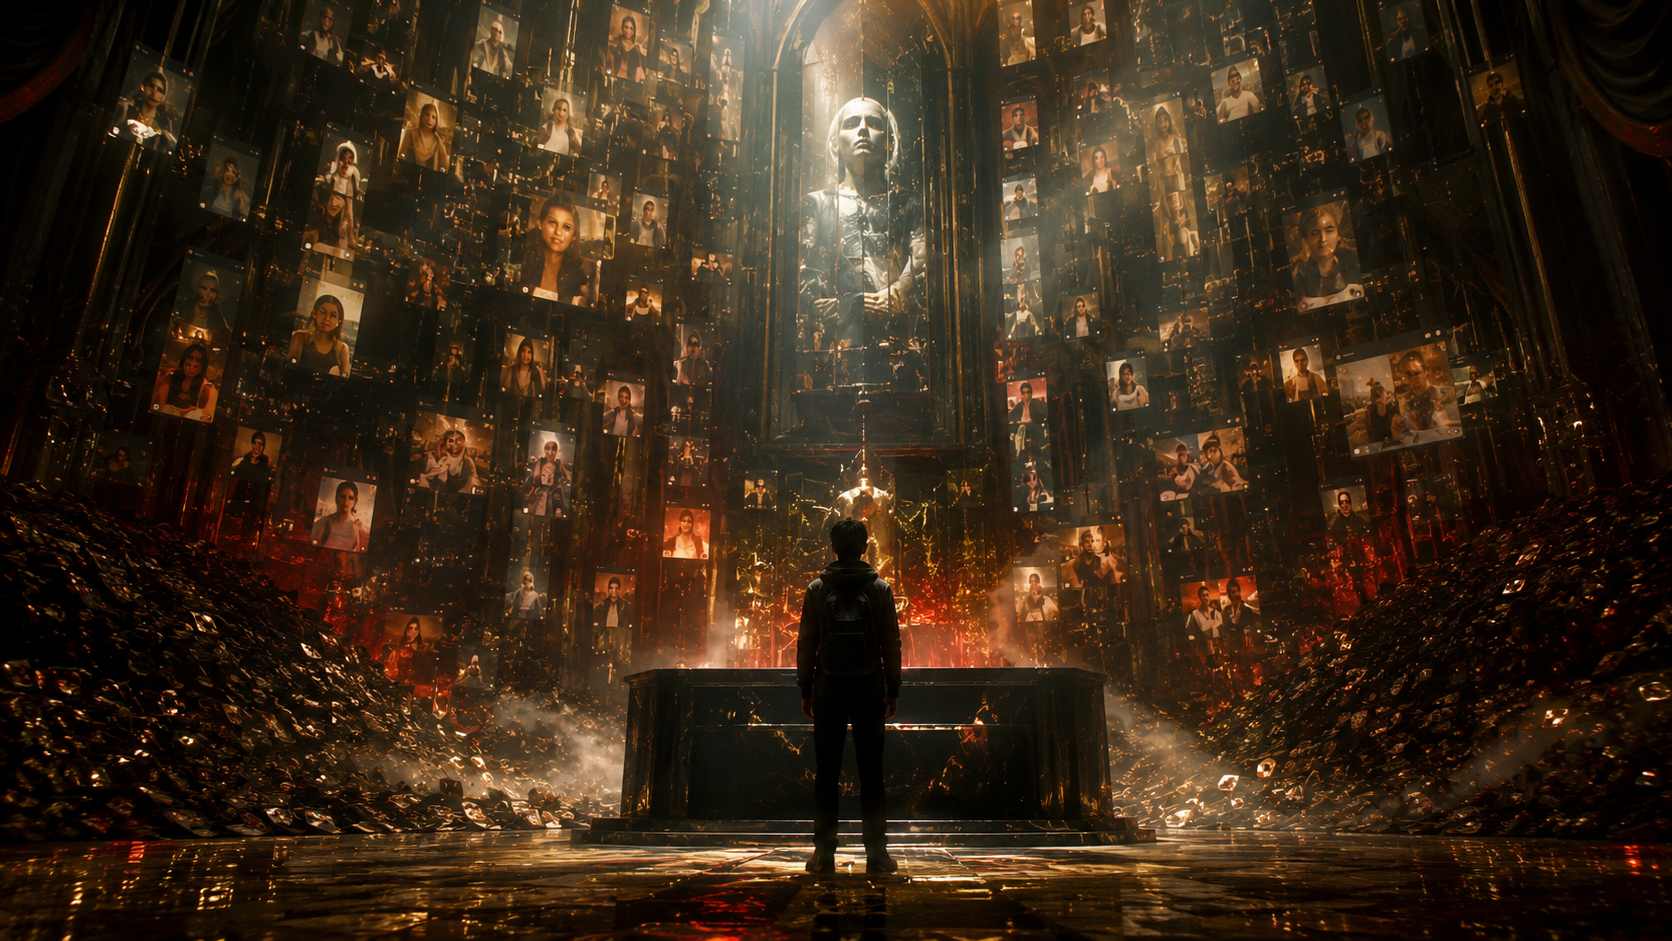
\includegraphics[keepaspectratio,alt={Chapter 01 narrative illustration}]{../assets/generated/illustrations/01_the-free-trap_scene.png}}
\caption{Chapter 01 narrative illustration}
\end{figure}

\begin{figure}
\centering
\pandocbounded{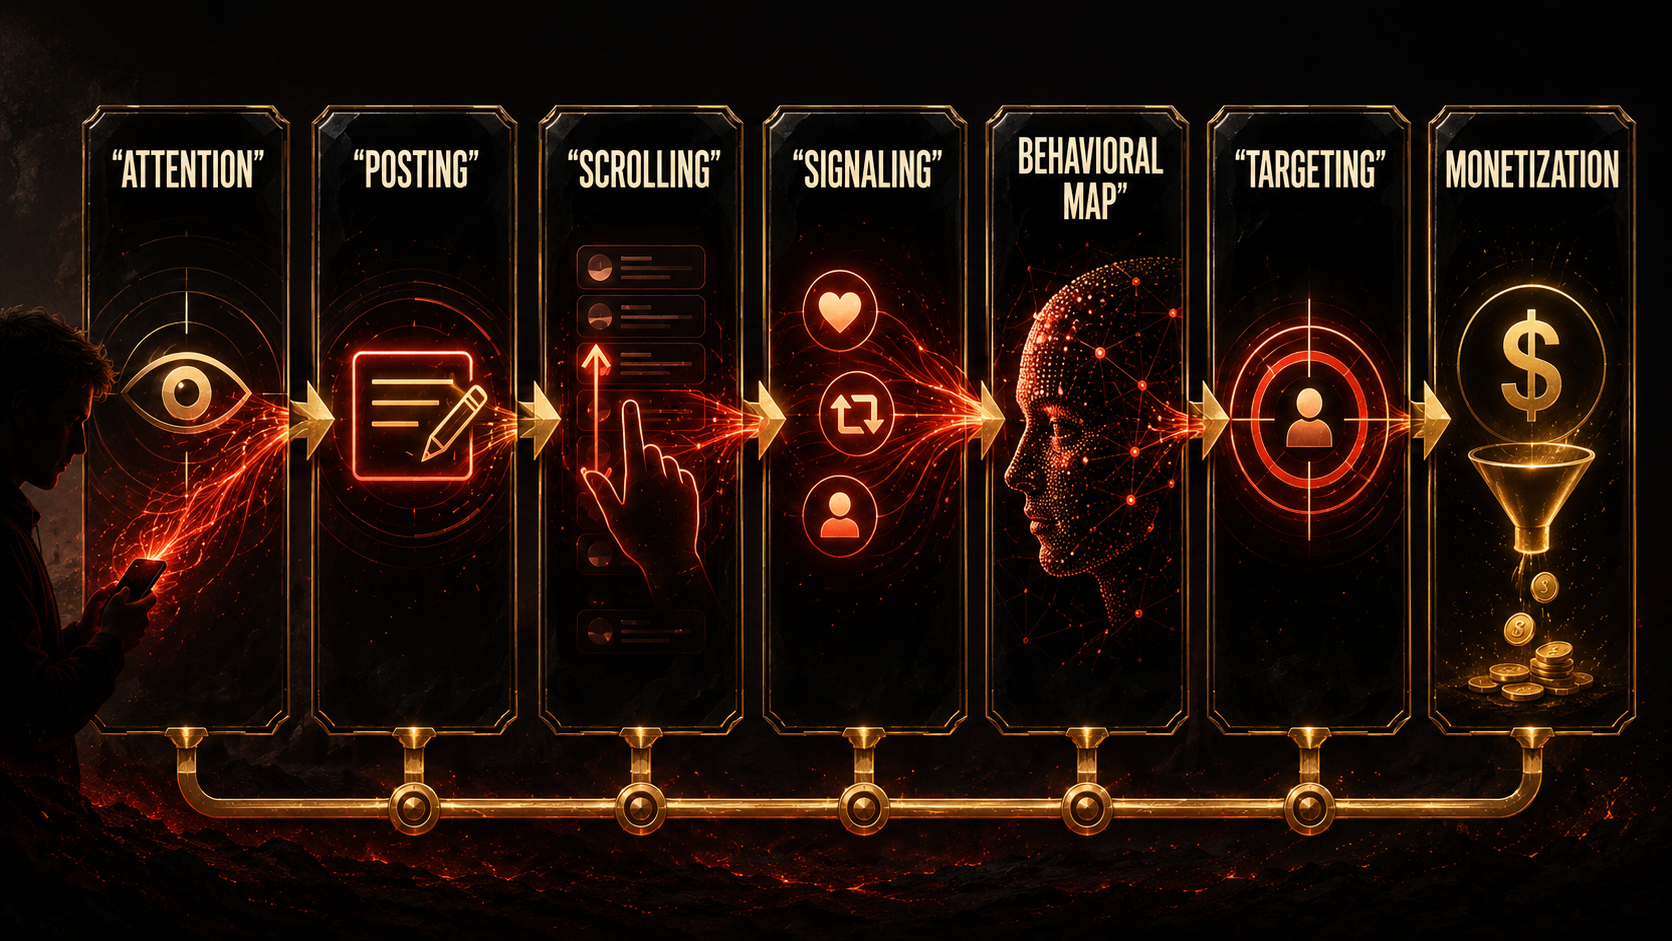
\includegraphics[keepaspectratio,alt={Chapter 01 infographic}]{../assets/generated/infographics/01_the-free-trap_infographic_a.png}}
\caption{Chapter 01 infographic}
\end{figure}

And because the culture normalized all of this during the rise of social
media, the later move into AI felt much less shocking than it should
have. By then, billions of people had already been trained to surrender
intimate expression in exchange for convenience, visibility, and ambient
belonging. The harvest was already happening. The public just did not
call it harvest.

That is why the free trap is not a nostalgia chapter. It is the
foundation chapter. If modern life had not already been privatized into
platforms, the later enclosure of intelligence would have looked more
absurd. The bridge from social media to AI is not a weird leap. It is
almost painfully direct. First the platforms map human behavior. Then
the archive becomes training material. Then the outputs return to
society as synthetic assistants, search layers, reasoning tools, and
replacement pressure.

The continuity is brutal once you see it.

\begin{figure}
\centering
\pandocbounded{
\includegraphics[keepaspectratio,alt={Chapter 01 narrative illustration B}]{../assets/generated/illustrations/01_the-free-trap_scene_b.png}}
\caption{Chapter 01 narrative illustration B}
\end{figure}

We thought we were building profiles.

We were building the field.

We thought we were networking.

We were feeding instrumentation.

We thought the app was a product.

The real product was a persistent, scalable model of us.

\begin{figure}
\centering
\pandocbounded{
\includegraphics[keepaspectratio,alt={Chapter 01 territorial extraction infographic}]{../assets/generated/infographics/01_the-free-trap_infographic_b.png}}
\caption{Chapter 01 territorial extraction infographic}
\end{figure}

And that is the point where the passive-intermediary story starts to
fall apart. A system that ranks exposure, tunes visibility, nudges
desire, profiles weakness, and monetizes emotional response is not just
a neutral wall on which strangers happen to speak. It is an active
environment. A governed environment. A behavioral landlord.

That shift matters for the reforms waiting at the end of this book.
Because if sovereign-scale platforms are really behavioral
infrastructure, then legal frameworks built around the fantasy of
passivity start looking obsolete on contact. You cannot keep giving
feudal power the liability profile of a bulletin board.

But before law catches up, culture has to catch up.

And culture still needs a cleaner sentence than most public debate
offers.

Here it is:

The feed did not go wrong by accident.

The feed was profitable because it turned human life into observability.

Everything after that follows from the same design logic.

\subsection{Research Basis}\label{research-basis}

This chapter adapts the documentary argument developed in the research
paper
\href{../../papers/html/01_social-networks-data-capture_paper.html}{\textbf{Chapter
01: Social Networks as Infrastructure for Free Data Capture}}. The PDF
version is
\href{../../papers/pdf/01_social-networks-data-capture_paper/01_social-networks-data-capture_paper.pdf}{here}.
That paper grounds the case in the FTC record, Facebook/Meta governance
history, and the platform business model of persistent extraction.

\subsection{Next}\label{next}

Once behavior can be captured, it can also be steered. The next chapter
leaves surveillance behind and moves into the psychic bill: what it
feels like to grow up inside systems that learn which forms of
insecurity keep us watching.

\end{document}
